\documentclass[aspectratio=1610, 9pt]{beamer}
\setbeamertemplate{section in toc}[sections numbered]
\setbeamertemplate{subsection in toc}{\hspace{1em}\inserttocsectionnumber.\inserttocsubsectionnumber.~\inserttocsubsection\par}

\linespread{1.3}
\usetheme{default}

\usepackage{mathpazo}
\renewcommand{\familydefault}{\rmdefault}

\usepackage{graphicx}
\usepackage{amsmath}
\usepackage{amsthm}
\usepackage{amsfonts} 
\usepackage{mathtools}
\usepackage{bbm}
\usepackage{tikz}
\usepackage[normalem]{ulem}
\usepackage[dvipsnames]{xcolor}
\usepackage{setspace}
\usepackage{array}
\usepackage{booktabs}
\usepackage{caption}
\usepackage{subcaption}
\usepackage{dsfont}
\usepackage{natbib}
\usepackage{appendixnumberbeamer}

\usepackage{threeparttable}
\usepackage{booktabs}
\usepackage{multirow}
\newcommand{\sym}[1]{\ifmmode^{#1}\else\(^{#1}\)\fi}

\bibliographystyle{apalike}
\usepackage{hyperref}
\hypersetup{
    colorlinks=true,
    linkcolor=blue,
    urlcolor=blue,
    citecolor=blue,
}
\setbeamersize{text margin left=0.8cm, text margin right = 5mm}
\newtheorem{assumption}{Assumption}

% \setbeamertemplate{theorems}[numbered]
% \setbeamertemplate{footline}[frame number]

\newcommand{\indep}{\rotatebox[origin=c]{90}{$\models$}}
\newcommand\independent{\protect\mathpalette{\protect\independenT}{\perp}}
\def\independenT#1#2{\mathrel{\rlap{$#1#2$}\mkern2mu{#1#2}}}



\title[Chen 2025]{Difference-in-Differences in the Presence of Mediators}

\author{Kyunghoon Ban, Zhengrun Chen, D\'esir\'e K\'edagni}




\begin{document}
\maketitle

\begin{frame}{Introduction}

 

\tikzset{every picture/.style={line width=0.75pt}} %set default line width to 0.75pt        
\centering
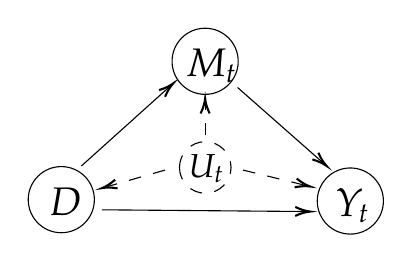
\begin{tikzpicture}[x=0.55pt,y=0.55pt,yscale=-0.9,xscale=0.9]
%uncomment if require: \path (0,563); %set diagram left start at 0, and has height of 563

%Shape: Circle [id:dp7073968717020449] 
\draw   (162.72,320.14) .. controls (162.72,306.81) and (173.53,296) .. (186.86,296) .. controls (200.19,296) and (211,306.81) .. (211,320.14) .. controls (211,333.47) and (200.19,344.28) .. (186.86,344.28) .. controls (173.53,344.28) and (162.72,333.47) .. (162.72,320.14) -- cycle ;
%Shape: Circle [id:dp9930267514584348] 
\draw   (373.72,321.14) .. controls (373.72,307.81) and (384.53,297) .. (397.86,297) .. controls (411.19,297) and (422,307.81) .. (422,321.14) .. controls (422,334.47) and (411.19,345.28) .. (397.86,345.28) .. controls (384.53,345.28) and (373.72,334.47) .. (373.72,321.14) -- cycle ;
%Shape: Circle [id:dp011069809067829839] 
\draw   (267.72,219.14) .. controls (267.72,205.81) and (278.53,195) .. (291.86,195) .. controls (305.19,195) and (316,205.81) .. (316,219.14) .. controls (316,232.47) and (305.19,243.28) .. (291.86,243.28) .. controls (278.53,243.28) and (267.72,232.47) .. (267.72,219.14) -- cycle ;
%Straight Lines [id:da21936795338565052] 
\draw    (201.55,295.55) -- (267.06,236.62) ;
\draw [shift={(268.55,235.28)}, rotate = 138.03] [color={rgb, 255:red, 0; green, 0; blue, 0 }  ][line width=0.75]    (10.93,-3.29) .. controls (6.95,-1.4) and (3.31,-0.3) .. (0,0) .. controls (3.31,0.3) and (6.95,1.4) .. (10.93,3.29)   ;
%Straight Lines [id:da5519235989627802] 
\draw    (216.55,327.55) -- (366.55,328.81) ;
\draw [shift={(368.55,328.83)}, rotate = 180.48] [color={rgb, 255:red, 0; green, 0; blue, 0 }  ][line width=0.75]    (10.93,-3.29) .. controls (6.95,-1.4) and (3.31,-0.3) .. (0,0) .. controls (3.31,0.3) and (6.95,1.4) .. (10.93,3.29)   ;
%Straight Lines [id:da8228607660966583] 
\draw    (315.55,238.28) -- (379.05,294.23) ;
\draw [shift={(380.55,295.55)}, rotate = 221.38] [color={rgb, 255:red, 0; green, 0; blue, 0 }  ][line width=0.75]    (10.93,-3.29) .. controls (6.95,-1.4) and (3.31,-0.3) .. (0,0) .. controls (3.31,0.3) and (6.95,1.4) .. (10.93,3.29)   ;
%Shape: Circle [id:dp9208138828826622] 
\draw  [color={rgb, 255:red, 0; green, 0; blue, 0 }  ,draw opacity=1 ][dash pattern={on 4.5pt off 4.5pt}] (273.13,296.64) .. controls (273.13,286.25) and (281.56,277.83) .. (291.95,277.83) .. controls (302.34,277.83) and (310.76,286.25) .. (310.76,296.64) .. controls (310.76,307.03) and (302.34,315.45) .. (291.95,315.45) .. controls (281.56,315.45) and (273.13,307.03) .. (273.13,296.64) -- cycle ;
%Straight Lines [id:da31773929683951785] 
\draw [color={rgb, 255:red, 0; green, 0; blue, 0 }  ,draw opacity=1 ] [dash pattern={on 4.5pt off 4.5pt}]  (291.86,273) -- (291.86,248.28) ;
\draw [shift={(291.86,246.28)}, rotate = 90] [color={rgb, 255:red, 0; green, 0; blue, 0 }  ,draw opacity=1 ][line width=0.75]    (10.93,-3.29) .. controls (6.95,-1.4) and (3.31,-0.3) .. (0,0) .. controls (3.31,0.3) and (6.95,1.4) .. (10.93,3.29)   ;
%Straight Lines [id:da14424295630385497] 
\draw [color={rgb, 255:red, 0; green, 0; blue, 0 }  ,draw opacity=1 ] [dash pattern={on 4.5pt off 4.5pt}]  (262.55,298.55) -- (218.47,311.18) ;
\draw [shift={(216.55,311.73)}, rotate = 344.01] [color={rgb, 255:red, 0; green, 0; blue, 0 }  ,draw opacity=1 ][line width=0.75]    (10.93,-3.29) .. controls (6.95,-1.4) and (3.31,-0.3) .. (0,0) .. controls (3.31,0.3) and (6.95,1.4) .. (10.93,3.29)   ;
%Straight Lines [id:da5459544581240827] 
\draw [color={rgb, 255:red, 0; green, 0; blue, 0 }  ,draw opacity=1 ] [dash pattern={on 4.5pt off 4.5pt}]  (319.55,298.55) -- (366.61,310.08) ;
\draw [shift={(368.55,310.55)}, rotate = 193.76] [color={rgb, 255:red, 0; green, 0; blue, 0 }  ,draw opacity=1 ][line width=0.75]    (10.93,-3.29) .. controls (6.95,-1.4) and (3.31,-0.3) .. (0,0) .. controls (3.31,0.3) and (6.95,1.4) .. (10.93,3.29)   ;

% Text Node
\draw (176,310) node [anchor=north west][inner sep=0.75pt]   [align=left] {{\Large $D$}};
% Text Node
\draw (385,310) node [anchor=north west][inner sep=0.75pt]   [align=left] {{\Large $Y_t$}};
% Text Node
\draw (276,208) node [anchor=north west][inner sep=0.75pt]   [align=left] {{\Large $M_t$}};
% Text Node
\draw (278,285) node [anchor=north west][inner sep=0.75pt]   [align=left] {{\large $U_t$}};


\end{tikzpicture}





\vspace{0.2cm}

\begin{itemize}
    \item Causal mediation in DiD setting: 
    \begin{itemize}
        \item[-] Two periods: $t=0$ (before treatment) and $t=1$ (after treatment)
        \item[-] A binary treatment $D$, a mediator $M_t$, and an outcome $Y_t$ 
        \item[-] $U_t$ is a vector of confounders
    \end{itemize}
    
    \vspace{0.1cm}
    \item Goal: Disentangle the direct effects and indirect effects of $D$ on $Y_t$
    
      \vspace{0.1cm}
    \item Common practice: Treat $M_t$ as a control variable and include it in the regression
    
    \begin{itemize}
        \item[-] Bad controls (Pearl, 1995; Angrist and Pischke, 2009)
    \end{itemize}

\end{itemize}

\end{frame}




\begin{frame}{Literature}

\begin{itemize}
  \item Mediation analysis (Imai et al., 2010; Huber, 2014; Acharya et al., 2016)\\ Sequential ignorability: (1)\ $D \ \indep\ \big( Y(d^\prime , m), M(d) \big) $,  \hspace{0.1cm} (2)  $ M(d) \ \indep\ Y(d^\prime,m) \mid D=d$
   
        % \begin{itemize}
        %     \item[(i)] $D \ \indep\ \big( Y(d^\prime , m), M(d) \big)$  
        %     \item[(ii)] $M(d) \ \indep\ Y(d^\prime,m) \mid D$
        % \end{itemize}
        \vspace{0.3cm}

    \item DiD with a binary mediator (Deuchert et al., 2019; Schenk, 2024)
        \begin{itemize}
         \item[-] Stratify the population into finite types by potential mediators
         \item[-] PTs hold for D conditional on types, \ PTs hold for $M_1(0)$ conditional on $D=0$
            \item[-] Monotonicity, Homogeneous mediator effects across types, ...
        \end{itemize} 
        \vspace{0.1cm}

        \textbf{This paper}: Allow PTs to be violated, and the mediators to be continuous
        \vspace{0.3cm}
    \item DiD with exogenous covariates (Caetano and Callaway, 2024)
    \begin{itemize}
        \item[-] Parallel trends hold  conditional on covariates: $\mathbb{E} [\Delta Y(0)\mid D=1, X_1,X_0,Z]=\mathbb{E} [\Delta Y(0)\mid D=0, X_1,X_0,Z].$  
        \\ \vspace{0.1cm}
        \ \ \textit{``This implicitly rules out bad controls''.}
    
        \end{itemize}
        
        \begin{itemize}
          
        \item[-] TWFE regression fails even with two time periods
    \end{itemize}
        \vspace{0.1cm}

    \textbf{This paper}: TWFE regression again not works in the presence of \textit{``bad controls''}; Propose the assumptions s.t. direct effects and indirect effects can be identified.
\end{itemize}
    
\end{frame}



\begin{frame}{Setup}
Two-period and two-group model: $t\in \{0,1\}, D_i\in\{0,1\} $
\[ 
\begin{cases}
     Y_{it} = \textcolor{blue}{\theta_i} \hspace{0.1em} t  \hspace{0.06em} D_i   +{\beta_{it}} \hspace{0.1em} M_{it}+ \textcolor{red}{\lambda_i}+\eta_t+{U_{it}} \\
     M_{it} = {\alpha_i}\hspace{0.1em} t \hspace{0.06em} D_i   + \textcolor{red}{\gamma_i} +\delta_t +{V_{it}} \\
     D_i = h(\textcolor{red}{\lambda_i},\textcolor{red}{\gamma_i},\textcolor{red}{\varepsilon_i})
\end{cases}
\]

 % \vspace{0.2cm}

\begin{block}{Assumption 1 (Exogenous Fixed Effects)}
    $(\textcolor{red}{\lambda_i},\textcolor{red}{\gamma_i},\textcolor{red}{\varepsilon_i}) \ \indep\ \left( {\alpha_i}, \{{V_{it}},{\beta_{it}}, {U_{it}}\}_{t\in\{0,1\}} \right) $
\end{block}


\begin{block}{Assumption 2 (Conditional Independence)}

$   \left( {\alpha_i}, \{{V_{it}}\}_{t\in\{0,1\}}\right) \ \indep\ \left(\{ {\beta_{it}},{U_{it}}\}_{t\in\{0,1\}}\right) \mid (\textcolor{red}{\lambda_i},\textcolor{red}{\gamma_i},\textcolor{red}{\varepsilon_i})$
    
\end{block}

\vspace{0.3cm}

\begin{itemize}
    \item DiD version of sequential ignorability.
    \item $\theta_i$ is allowed to depend on $(M_{i0},M_{i1})$ as well as fixed effects
    \item Also assume SUTVA, No Anticipation ($\theta_{i0}=0,\alpha_{i0}=0$), and Overlap condition.
\end{itemize}

\end{frame}




\begin{frame}{Setup}
Potential outcome:
         $$Y_{it}(d,M_{it}(d))=\theta_i \hspace{0.1em} t \hspace{0.05em} d   + \beta_{it}\hspace{0.1em} M_{it}(d)+\lambda_i+\eta_t + U_{it}$$
Potential mediator:
        $$M_{it}(d)=\alpha_i \hspace{0.1em} t\hspace{0.05em} d  + \gamma_i +\delta_t +V _{it}$$

Avg. treatment effect on the treated (ATT): $$\mathbb{E}[Y_1(\textcolor{red}{1},M_{i1}(\textcolor{red}{1}))-Y_1(\textcolor{blue}{0},M_{i1}(\textcolor{blue}{0}))\mid D_i=1]=\mathbb{E}[\theta_i\mid D_i=1] +\mathbb{E}[\alpha_i]\mathbb{E}[\beta_{i1}]$$

Avg. direct effect on the treated (ADTT):
$$\mathbb{E}[Y_1(\textcolor{red}{1},M_{i1}(1))-Y_1(\textcolor{blue}{0},M_{i1}(1))\mid D_i=1]=\mathbb{E}[\theta_i \mid D_i=1]$$

Avg. indirect effects on the treated (AITT): 
$$\mathbb{E}[Y_1(0,M_{i1}(\textcolor{red}{1}))-Y_1(0,M_{i1}(\textcolor{blue}{0}))\mid D_i=1]=\mathbb{E}[\alpha_i]\mathbb{E}[\beta_{i1}]$$

\end{frame}


\begin{frame}{Total Effects} \label{Bias}

\textbf{Does the standard DiD estimand/ TWFE estimand identify the total effects?}
 $$\tau^{DiD}\equiv \mathbb{E}[\Delta Y_i\mid D_i=1]-\mathbb{E}[\Delta Y_i\mid D_i=0]$$  where $\Delta Y_i \equiv  Y_{i1} - Y_{i0}.$ \vspace{0.5cm}\\

 % \pause

\only<1>{
\begin{itemize}
     \item The standard PTs may not hold
        \begin{eqnarray*}
         \mathbb{E}[\Delta Y_{i}(0)\mid D_i=1]-\mathbb{E}[\Delta Y_{i}(0)\mid D_i=0]
            & =  & \textcolor{red}{\mathbb{E}(\beta_{i1}-\beta_{i0}) \cdot \big( \mathbb{E}[\gamma_i\mid D_i=1]-\mathbb{E}[\gamma_i\mid D_i=0]\big)}
   \end{eqnarray*} where $ \Delta Y_i(0) \equiv Y_{i1}(0,M_{i1}(0))- Y_{i0}(0,M_{i0}(0)).$
   \vspace{0.2cm}
% \pause
    \item Under Assumption 1 and 2, 
    \begin{eqnarray*}
         \tau^{DiD} &=& \textcolor{blue}{\mathbb{E}[\theta_i\mid D_i=1]}+\textcolor{blue}{\mathbb{E}[\alpha_i]\cdot \mathbb{E}(\beta_{i1})}+  \textcolor{red}{\mathbb{E}(\beta_{i1}-\beta_{i0}) \cdot \big( \mathbb{E}[\gamma_i\mid D_i=1]-\mathbb{E}[\gamma_i\mid D_i=0]\big)}\\
         & = &  \textcolor{blue}{\text{ avg. direct effect }} + \textcolor{blue}{\text{ avg. indirect effect }} +  \textcolor{red}{\text{ bias term }}
    \end{eqnarray*}
      
\end{itemize}
}

\only<2>{
\vspace{-0.4cm}
\centering
 \begin{minipage}{0.5\textwidth}
        
\includegraphics[width=\linewidth]{Graph_Mediator/theta_total_sim_new.pdf} 
        
        \vspace{-0.1cm}
        \captionof{figure}{TWFE estimator for the direct effect}
    \end{minipage}
    
    \vspace{-0.6cm}
    \raggedright \hyperlink{DGP}{\beamergotobutton{DGP}}

}
    
    
\end{frame}



\begin{frame}{Direct Effects}
% \vspace{0.3cm}

\textbf{Does the TWFE regression conditional on $M_{it}$ work?}
$$Y_{it}=\ \pi_1\hspace{0.1em} t \hspace{0.05em}D_{i}+\pi_2 \hspace{0.1em} M_{it}+\lambda_{i}+\eta_{t}+e_{it}\ \qquad t\in\{0,1\}$$
% \vspace{0.1cm}

\only<1>{
\begin{itemize}
    \item  Under Assumption 1 and 2, 
     \begin{eqnarray*}
        \pi_1 & = & \textcolor{blue}{\mathbb{E}[\theta_{i}\mid D_{i}=1]}\\
        & + & \textcolor{red}{\mathbb{E}(\beta_{i1}-\beta_{i0})\left(\frac{Cov(D_{i},\gamma_{i})}{Var(\tilde{D}_{i})}-\frac{\mathbb{E}(\alpha_{i})Cov(\Delta M_{i},M_{i0})}{Var(\widetilde{\Delta M_i})}\right)}\\
        & + & \textcolor{red}{ \frac{\mathbb{E}(\alpha_{i})}{Var(\widetilde{\Delta M_{i}})}\Big(\mathbb{E}(\alpha_{i})Cov(D_{i},\theta_{i}D_{i})-Cov(\Delta M_{i},\theta_{i}D_{i})\Big)}
     \end{eqnarray*}

     If $\mathbb{E}(\beta_{i1})=\mathbb{E}(\beta_{i0})$ and $\theta_{i}\ \indep\ (\alpha_{i},V_{i0},V_{i1})$, then $\pi_1$ can recover ADTT.
\end{itemize}
}
\pause

\only<2>{
\vspace{-0.9cm}
\centering
 \begin{minipage}{0.5\textwidth}
        
\includegraphics[width=\linewidth]{Graph_Mediator/theta_direct_sim_new.pdf} 
        
        \vspace{-0.1cm}
        \captionof{figure}{TWFE estimator for the direct effect}
    \end{minipage}
}

\end{frame}



% \begin{frame}{Direct Effects}
% \centering
%     \begin{minipage}{0.49\textwidth}
%         
\includegraphics[width=\linewidth]{Graph/theta_total_sim.pdf}
%         \captionof{figure}{TWFE estimator for the total effect}
%     \end{minipage}\hfill
%     \begin{minipage}{0.49\textwidth}
%         
\includegraphics[width=\linewidth]{Graph/theta_direct_sim.pdf}
%         \captionof{figure}{TWFE estimator for the direct effect}
%     \end{minipage}
% \end{frame}


\begin{frame}{Direct Effects}

\textbf{How about conditional DiD estimand?}\\
\vspace{0.1cm}
% For $(m_0,m_1)\in \boldsymbol{\mathcal{M}}_{0}\cap \boldsymbol{\mathcal{M}}_{1}$, 
$$\tau^{DiD}(m_0,m_1)\equiv \mathbb E[\Delta Y_i \mid D_i=1, M_{i0}=m_0, M_{i1}=m_1]- \mathbb E[\Delta Y_i \mid D_i=0, M_{i0}=m_0, M_{i1}=m_1]$$ 
 

 
% \begin{block}{Proposition}
%     Under Assumptions 1 and 2, the average conditional direct effect on the treated is identified.
%     \begin{eqnarray*}
%      \mathbb{E} [\ \theta_i\mid D_i=1, M_{i1},M_{i0}]
%     & = & \mathbb E[\Delta Y_i \mid D_i=1, M_{i1}, M_{i0}]- \mathbb E[\Delta Y_i \mid D_i=0, M_{i1}, M_{i0}]
% \end{eqnarray*}
% \end{block}

\pause

\begin{block}{Proposition 1}
    Under Assumptions 1 and 2, the conditional average direct effect on the treated is identified
   $$   \tau^{DiD}(m_0,m_1)
    \ = \ \mathbb{E} [\ \theta_i\mid D_i=1, M_{i0}=m_0,M_{i1}=m_1]\ \equiv \ CADTT $$

% \vspace{0.1cm}
 And, the average direct effect on the treated is identified
    $$ \mathbb{E}\big[ \tau^{DiD}(M_{i1},M_{i0}) \big| D_i =1\big]
    \ =  \ \mathbb{E} [\ \theta_i\mid D_i=1] \ \equiv \ ADTT $$
    % &=& \mathbb{E} \big[ \mathbb E[\Delta Y_i \mid D_i=1, M_{i1}, M_{i0}]- \mathbb E[\Delta Y_i \mid D_i=0, M_{i1}, M_{i0}] \big| D_i=1 ,\big]
\end{block}

\begin{itemize}
    \item \textbf{Conditional DiD estimand} identifies the direct effects even when \textbf{conditional PTs} is violated.
    \item This result also holds for discrete mediators
\end{itemize}
\end{frame}




\begin{frame}{Indirect Effects}

    \begin{block}{Assumption 3 (Stable average mediator effect)}
    $\mathbb E[\beta_{i1}]=\mathbb E[\beta_{i0}]$
\end{block}
\vspace{0.5cm}
Under Assumptions 1-3, 
\textcolor{blue}{$\tau^{DiD}=\mathbb E[\theta_i \vert D_i=1] +\mathbb E[\beta_{i}] \cdot \mathbb E[\alpha_i]$}.

\vspace{0.5cm}

\begin{block}{Proposition 2}
    Suppose $\mathbb{E}[\Delta M_i \mid D_i=1]-\mathbb{E}[\Delta M_i \mid D_i=0] \neq 0$. Given Assumptions 1-3, $\mathbb{E}(\alpha_i)$ and $\mathbb E[\beta_{i1}]$ are identified: \begin{eqnarray*}
    \mathbb{E}[\alpha_i]& = & \mathbb{E}[\Delta M_i \mid D_i=1]-\mathbb{E}[\Delta M_i \mid D_i=0]\\
        \mathbb E[\beta_{i1}] &=& \frac{\textcolor{blue}{\tau^{DiD}}-\textcolor{red}{\mathbb{E}\big[ \tau^{DiD}(M_{i1},M_{i0}) \big| D_i =1\big]} }{\mathbb{E}[\Delta M_i \mid D_i=1]-\mathbb{E}[\Delta M_i \mid D_i=0]}
    \end{eqnarray*}
\end{block}

\end{frame}

\begin{frame}{Empirical Example: Howard and Ornaghi (2021)}
\begin{itemize}
    \item  It studies the effects of Alcohol Prohibition in the early 20th century in the US.
    \vspace{0.1cm}
    \item \textbf{Local policy}: County-level Alcohol Prohibition
     \vspace{0.1cm}
     \item \textbf{Two periods}: 1900 vs 1910
          \vspace{0.1cm}
    \item \textbf{Treatment group}: early adopters vs \textbf{Control group}: late adopters
     \vspace{0.1cm}
    \item Prohibition (D) $\rightarrow$ Land values (M) $\uparrow$
    \begin{itemize}
\item[-] It raised amenity value, attracting people and raising land prices.
    \end{itemize}
     \vspace{0.1cm}
    \item Prohibition (D) $\rightarrow$ farm productivity (Y) $\uparrow$
    \begin{itemize}
    \item[-] Indirect: Higher land values $\rightarrow$ more collateral $\rightarrow$ expand access to credit $\rightarrow$ more farm investment
        \item[-] Direct: More sober worker, ...
    \end{itemize}

\end{itemize}

\vspace{0.3cm}

    \tikzset{every picture/.style={line width=0.75pt}} 
%set default line width to 0.75pt     
\centering
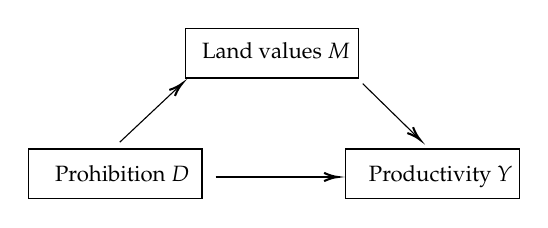
\begin{tikzpicture}[x=0.45pt,y=0.45pt,yscale=-1,xscale=1]
%uncomment if require: \path (0,563); %set diagram left start at 0, and has height of 563

%Flowchart: Process [id:dp21628664710052603] 
\draw   (122,228.82) -- (261.55,228.82) -- (261.55,268.82) -- (122,268.82) -- cycle ;
%Flowchart: Process [id:dp4932393895766205] 
\draw   (248,131.82) -- (387.55,131.82) -- (387.55,171.82) -- (248,171.82) -- cycle ;
%Flowchart: Process [id:dp9912179358547202] 
\draw   (377,228.82) -- (516.55,228.82) -- (516.55,268.82) -- (377,268.82) -- cycle ;
%Straight Lines [id:da6460170926979678] 
\draw    (195.55,223.28) -- (244.09,177.65) ;
\draw [shift={(245.55,176.28)}, rotate = 136.77] [color={rgb, 255:red, 0; green, 0; blue, 0 }  ][line width=0.75]    (10.93,-3.29) .. controls (6.95,-1.4) and (3.31,-0.3) .. (0,0) .. controls (3.31,0.3) and (6.95,1.4) .. (10.93,3.29)   ;
%Straight Lines [id:da1914525523938091] 
\draw    (390.55,176.28) -- (435.12,219.88) ;
\draw [shift={(436.55,221.28)}, rotate = 224.37] [color={rgb, 255:red, 0; green, 0; blue, 0 }  ][line width=0.75]    (10.93,-3.29) .. controls (6.95,-1.4) and (3.31,-0.3) .. (0,0) .. controls (3.31,0.3) and (6.95,1.4) .. (10.93,3.29)   ;
%Straight Lines [id:da48066913310142545] 
\draw    (272.55,251.28) -- (368.55,251.28) ;
\draw [shift={(370.55,251.28)}, rotate = 180] [color={rgb, 255:red, 0; green, 0; blue, 0 }  ][line width=0.75]    (10.93,-3.29) .. controls (6.95,-1.4) and (3.31,-0.3) .. (0,0) .. controls (3.31,0.3) and (6.95,1.4) .. (10.93,3.29)   ;

% Text Node
\draw (142,240) node [anchor=north west][inner sep=0.5pt]   [align=left] {{\footnotesize Prohibition $D$}};
% Text Node
\draw (260,142) node [anchor=north west][inner sep=0.5pt]   [align=left] {{\footnotesize Land values $M$}};
% Text Node
\draw (394,240) node [anchor=north west][inner sep=0.5pt]   [align=left] {{\footnotesize Productivity $Y$}};
\end{tikzpicture}
    
\end{frame}



\begin{frame}{Empirical Example: Howard and Ornaghi (2021)} \label{ADTT_estimate}
\vspace{-0.4cm}
\begin{table}
\centering
\begin{threeparttable}

\label{tab:estimates}
\renewcommand{\arraystretch}{0.98}
\setlength{\tabcolsep}{9pt}

\begin{tabular}{lccc}
\toprule
& TWFE
& \multicolumn{2}{c}{Doubly Robust} \\
\cmidrule(lr){3-4}
& & Linear + Logit & Quadratic + Logit \\
& (1) & (2) & (3) \\
\midrule

$D \to Y$ (Total)
& 0.093\sym{*}
& 0.132\sym{***}
& 0.115\sym{***} \\
& (0.037)
& (0.040)
& (0.041) \\[3pt]

$D \to Y$ (Direct)
& 0.065
& 0.103\sym{**}
& 0.105\sym{**} \\
& (0.035)
& (0.046)
& (0.046) \\[3pt]

$D \to M$
& 0.056\sym{*}
& 0.135\sym{***}
& 0.141\sym{***} \\
& (0.022)
& (0.027)
& (0.026) \\[3pt]

$M \to Y$
& 0.497\sym{***}
& 0.218\sym{*}
& 0.063 \\
& (0.076)
& (0.139)
& (0.177) \\[3pt]

$D \to M \to Y$ (Indirect)
& 0.028\sym{***}
& 0.031\sym{*}
& 0.009 \\
& (0.013)
& (0.020)
& (0.027) \\

\midrule
Baseline controls & Yes & Yes & Yes \\
Observations      & 4{,}684 & 4{,}684 & 4{,}684 \\
\bottomrule
\end{tabular}
\end{threeparttable}
\end{table}
\end{frame}





\begin{frame}{Summary}

\begin{itemize}

        \item Consider the identification of causal effects in DiD models in the presence of mediators.
        \item Propose assumptions under which we can identify the average direct/indirect effects.
        \item Result can be extended to multivariate mediators and a staggered adoption setting.
    \end{itemize}

    
\end{frame}




\appendix

\section{Appendix}



\begin{frame}{Direct Effects}

\begin{block}{Lemma}
   Assumptions 1 and 2 imply that $  \big(\ \textcolor{blue}{\{\beta_{it},U_{it}\}_{t=0,1}} \ \big) \ \indep\ \big(\ \textcolor{red}{\alpha_i,\{V_{it}\}_{t=0,1},\lambda_i,\gamma_i,\varepsilon_i}\ \big)$
\end{block}

\begin{align*}
    &\ \mathbb E[\Delta Y_i \mid D_i=1, M_{i0}=m_0, M_{i1}=m_1]- \mathbb E[\Delta Y_i \mid D_i=0, M_{i0}=m_0, M_{i1}=m_1]\\
    =&\ \mathbb E[\theta_i \mid D_i=1, M_{i1}=m_1, M_{i0}=m_0]\\
    & + \mathbb E\big[\textcolor{blue}{\beta_{i1}}m_{1}-\textcolor{blue}{\beta_{i0}}m_{0}+\eta_1-\eta_0 + \textcolor{blue}{U_{i1}}-\textcolor{blue}{U_{i0}}\mid h(\textcolor{red}{\lambda_i}, \textcolor{red}{\gamma_i},\textcolor{red}{\varepsilon_i})=1, \textcolor{red}{\alpha_i}+\textcolor{red}{\gamma_i}+\delta_1+\textcolor{red}{V_{i1}}=m_1, \textcolor{red}{\gamma_i}+\delta_0+\textcolor{red}{V_{i0}}=m_0\big]\\
    & -\mathbb E\big[\textcolor{blue}{\beta_{i1}}m_{1}-\textcolor{blue}{\beta_{i0}}m_{0}+\eta_1-\eta_0 + \textcolor{blue}{U_{i1}}-\textcolor{blue}{U_{i0}}\mid h(\textcolor{red}{\lambda_i},\textcolor{red}{\gamma_i},\textcolor{red}{\varepsilon_i})=0, \textcolor{red}{\gamma_i}+\delta_1+\textcolor{red}{V_{i1}}=m_1, \textcolor{red}{\gamma_i}+\delta_0+\textcolor{red}{V_{i0}}=m_0\big]\\
    =&\ \mathbb E[\theta_i \mid D_i=1, M_{i1}=m_1, M_{i0}=m_0]
\end{align*}
    
\end{frame}
\begin{frame}{Direct Effects}


\begin{itemize}
    \item Conditional PTs may fail

    \vspace{-0.6cm}

    
\begin{eqnarray*}
    && \mathbb{E} [\Delta Y_{i}(0) \mid D=1,M_{i0}=m_0,M_{i1}=m_1]
    -\mathbb E[\Delta Y_{i}(0) \mid D=0,M_{i0}=m_0,M_{i1}=m_1]\\
   & = &\textcolor{red}{ \mathbb E\big[ -\alpha_i\beta_{i1} \mid D_i=1,M_{i0}=m_0,M_{i1}=m_1\big]} \ = \ - \text{Indirect effects}
\end{eqnarray*}

\hspace{-0.6cm} $\tau^{DiD}(m_0,m_1)= \underbrace{\mathbb{E}(\theta_i+\alpha_i\beta_{i1}\mid D_i=1,M_{i0}=m_0,M_{i1}=m_1)}_\text{Conditional total treatment effect on the treated}
     + \underbrace{\textcolor{red}{\mathbb{E}[-\alpha_i\beta_{i1}\mid D_i=1,M_{i0}=m_0,M_{i1}=m_1]}}_\text{Differential in trends}$
\end{itemize}

\vspace{0.2cm}



\tikzset{every picture/.style={line width=0.75pt}} %set default line width to 0.75pt        
\centering
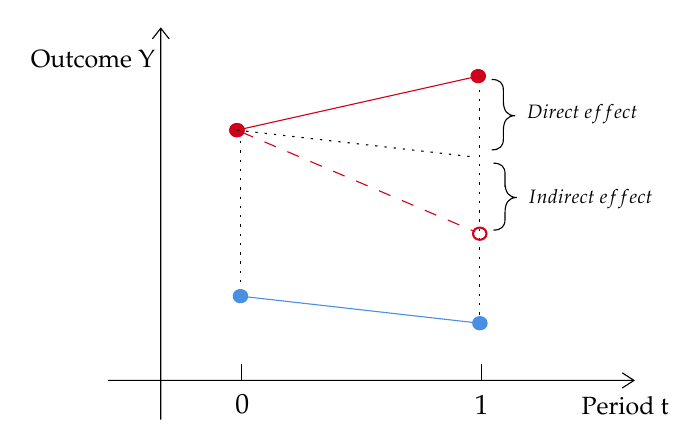
\begin{tikzpicture}[x=0.55pt,y=0.55pt,yscale=-1,xscale=1.1]
%uncomment if require: \path (0,503); %set diagram left start at 0, and has height of 503

%Straight Lines [id:da13121618667406865] 
\draw    (386.76,412.39) -- (386.76,401.71) ;
%Straight Lines [id:da8892828166920976] 
\draw    (243.22,412.39) -- (243.22,401.71) ;
%Straight Lines [id:da3145034554410573] 
\draw  [dash pattern={on 0.84pt off 2.51pt}]  (242.46,248.76) -- (242.46,359.98) ;
%Straight Lines [id:da38832706431548236] 
\draw  [dash pattern={on 0.84pt off 2.51pt}]  (385.54,215.07) -- (385.54,374.6) ;
%Straight Lines [id:da8789346811842831] 
\draw [color={rgb, 255:red, 74; green, 144; blue, 226 }  ,draw opacity=1 ]   (242.54,356.81) -- (385.54,374.6) ;
\draw [shift={(385.54,374.6)}, rotate = 7.09] [color={rgb, 255:red, 74; green, 144; blue, 226 }  ,draw opacity=1 ][fill={rgb, 255:red, 74; green, 144; blue, 226 }  ,fill opacity=1 ][line width=0.75]      (0, 0) circle [x radius= 4.02, y radius= 4.02]   ;
\draw [shift={(242.54,356.81)}, rotate = 7.09] [color={rgb, 255:red, 74; green, 144; blue, 226 }  ,draw opacity=1 ][fill={rgb, 255:red, 74; green, 144; blue, 226 }  ,fill opacity=1 ][line width=0.75]      (0, 0) circle [x radius= 4.02, y radius= 4.02]   ;
%Straight Lines [id:da4646523317448381] 
\draw [color={rgb, 255:red, 208; green, 2; blue, 27 }  ,draw opacity=1 ] [dash pattern={on 4.5pt off 4.5pt}]  (243.19,249.04) -- (382.72,314.47) ;
\draw [shift={(385.46,315.76)}, rotate = 25.12] [color={rgb, 255:red, 208; green, 2; blue, 27 }  ,draw opacity=1 ][line width=0.75]      (0, 0) circle [x radius= 4.02, y radius= 4.02]   ;
\draw [shift={(240.46,247.76)}, rotate = 25.12] [color={rgb, 255:red, 208; green, 2; blue, 27 }  ,draw opacity=1 ][line width=0.75]      (0, 0) circle [x radius= 4.02, y radius= 4.02]   ;
%Shape: Brace [id:dp003966146529122527] 
\draw   (392.55,260.7) .. controls (397.22,260.7) and (399.55,258.37) .. (399.55,253.7) -- (399.55,248.26) .. controls (399.55,241.59) and (401.88,238.26) .. (406.55,238.26) .. controls (401.88,238.26) and (399.55,234.93) .. (399.55,228.26)(399.55,231.26) -- (399.55,221.43) .. controls (399.55,216.76) and (397.22,214.43) .. (392.55,214.43) ;
%Shape: Brace [id:dp7768312624542486] 
\draw   (393.55,313.43) .. controls (398.22,313.43) and (400.55,311.1) .. (400.55,306.43) -- (400.55,302) .. controls (400.55,295.33) and (402.88,292) .. (407.55,292) .. controls (402.88,292) and (400.55,288.67) .. (400.55,282)(400.55,285) -- (400.55,276.43) .. controls (400.55,271.76) and (398.22,269.43) .. (393.55,269.43) ;
%Shape: Axis 2D [id:dp5923235078351863] 
\draw  (163.55,412.17) -- (477.55,412.17)(194.95,180.79) -- (194.95,437.88) (470.55,407.17) -- (477.55,412.17) -- (470.55,417.17) (189.95,187.79) -- (194.95,180.79) -- (199.95,187.79)  ;
%Straight Lines [id:da5859683456313953] 
\draw [color={rgb, 255:red, 208; green, 2; blue, 27 }  ,draw opacity=1 ]   (384.55,212.25) -- (317.39,228.8) -- (240.46,247.76) ;
\draw [shift={(240.46,247.76)}, rotate = 166.16] [color={rgb, 255:red, 208; green, 2; blue, 27 }  ,draw opacity=1 ][fill={rgb, 255:red, 208; green, 2; blue, 27 }  ,fill opacity=1 ][line width=0.75]      (0, 0) circle [x radius= 4.02, y radius= 4.02]   ;
\draw [shift={(384.55,212.25)}, rotate = 166.16] [color={rgb, 255:red, 208; green, 2; blue, 27 }  ,draw opacity=1 ][fill={rgb, 255:red, 208; green, 2; blue, 27 }  ,fill opacity=1 ][line width=0.75]      (0, 0) circle [x radius= 4.02, y radius= 4.02]   ;
%Straight Lines [id:da25196696287100573] 
\draw [color={rgb, 255:red, 0; green, 0; blue, 0 }  ,draw opacity=1 ] [dash pattern={on 0.84pt off 2.51pt}]  (240.46,247.76) -- (383.46,265.54) ;

% Text Node
\draw (380.82,420.43) node [anchor=north west][inner sep=0.75pt]   [align=left] {1};
% Text Node
\draw (444.72,420.94) node [anchor=north west][inner sep=0.75pt]  [font=\small] [align=left] {Period t};
% Text Node
\draw (237.99,420.02) node [anchor=north west][inner sep=0.75pt]   [align=left] {0};
% Text Node
\draw (115.78,193.51) node [anchor=north west][inner sep=0.75pt]  [font=\small] [align=left] {Outcome Y};
% Text Node
\draw (403.62,228.11) node [anchor=north west][inner sep=0.75pt]  [font=\scriptsize] [align=left] {$\displaystyle  \begin{array}{{>{\displaystyle}l}}
Direct\ effect\\
\end{array}$};
% Text Node
\draw (412.62,285.11) node [anchor=north west][inner sep=0.75pt]  [font=\scriptsize] [align=left] {$\displaystyle Indirect\ effect$};


\end{tikzpicture}





\end{frame}


\begin{frame}{Data Generating Process (DGP) for Simulation} \label{DGP}
$$
(\lambda_{i},\gamma_{i},\theta_{i},\alpha_{i})\sim\mathcal{N}\left(\left(\begin{array}{c}
1\\
1\\
0.6\\
1
\end{array}\right),\left(\begin{array}{cccc}
1 & 0.5 & 0.5 & 0\\
0.5 & 1 & 0.5 & 0\\
0.5 & 0.5 & 1 & 0.5\\
0 & 0 & 0.5 & 1
\end{array}\right)\right)
$$


\begin{itemize}
     \item $D_{i}=\mathds{1}\{\lambda_{i}+\gamma_{i}>\varepsilon_{i}\}$ where $\varepsilon_{i}\sim\mathcal{N}(2,1)$
     
    \item $(\beta_{i0},\beta_{i1})\sim\mathcal{N}\left(\left(\begin{array}{c}
3\\
1
\end{array}\right),
 \left(\begin{array}{cc}
1 & 0.5\\
0.5 & 1
\end{array}\right)\right)$

    \item $(U_{i0},U_{i1})\sim\mathcal{N}\left(\left(\begin{array}{c}
0\\
0
\end{array}\right),
\left(\begin{array}{cc}
1 & 0.5\\
0.5 & 1
\end{array}\right)\right), (V_{i0},V_{i1})\sim\mathcal{N}\left(\left(\begin{array}{c}
0\\
0
\end{array}\right),\left(\begin{array}{cc}
1 & 0.5\\
0.5 & 1
\end{array}\right)\right)$
 \item  $(\eta_{0},\eta_{1})=(0,1)$, $(\delta_{0}$, $\delta_{1})=(0,1)$.
   
\end{itemize}

\vspace{0.4cm}
\hyperlink{Bias}{\beamerreturnbutton{return}}

\end{frame}











\end{document}